\providecommand{\main}{..} 
\documentclass[\main/boa.tex]{subfiles}

\begin{document}

\section[Kombajn do uczenia maszynowego - MLR w praktyce]{Kombajn do uczenia maszynowego \\- MLR w praktyce}
\begin{minipage}[t]{0.915\textwidth}
	\center     
    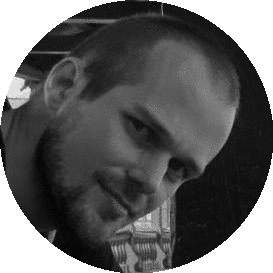
\includegraphics[width=60px]{img/workshops/czarno_biale/pzawistowski-crop.png} 
\end{minipage}

\begin{minipage}{0.915\textwidth}
\centering
{\bf \index[a]{Zawistowski Paweł} Paweł Zawistowski}
\end{minipage}

\vskip 0.3cm

\begin{affiliations}
\begin{minipage}{0.915\textwidth}
\centering
\large Politechnika Warszawska, Wydział EiTI, AdForm  \\[2pt]
\end{minipage}
\end{affiliations}

\vskip 0.8cm

\opiswarsztatu Kiedy coraz powszechniejsze staje się stosowanie mniej lub bardziej skomplikowanych modeli statystycznych, a liczba pakietów R'a z nowymi metodami i algorytmami ciągle wzrasta - dobrze mieć w zanadrzu narzędzie, które spina wszystkie etapy tworzenia modelu w jedną całość. Pakiet MLR jest takim właśnie "kombajnem", który może w znacznym stopniu ułatwić nam pracę. 

W ramach warsztatu zobaczymy jakie możliwości daje MLR przy tworzeniu różnego rodzaju modeli - przejdziemy przy tym kompletną ścieżkę, od wstępnego przygotowania danych, przez wybór odpowiedniej metody, strojenie parametrów, aż po diagnostykę i wizualizacje wyników.

\planwarsztatu
\begin{enumerate}
\item Omówienie możliwości pakietu MLR, przygotowanie środowiska.
\item Przygotowanie danych do rozwiązywania naszego zadania (klasyfikacja, regresja, ...).
\item Wybór modelu, strojenie parametrów.
\item Diagnostyka i wizualizacja wyników.
\item Rozszerzanie MLR o własny algorytm.
\item Inne ciekawe elementy pakietu, podsumowanie.
\end{enumerate}	 

\pakiety W ramach warsztatu korzystać będziemy z `mlr` oraz `tidyverse`. Udostępniony zostanie również obraz dockera ze wszystkim co potrzebne + RStudio.

\umiejetnosci\begin{enumerate}
	\item Ogólna znajomość zagadnień związanych z tworzeniem modeli statystycznych, umiejętność korzystania z R'a w stylu "tidyverse". 
	\item Podstawowa umiejętność korzystania z dockera.
\end{enumerate}

\wymagania Instalacja pakietów R lub ściągnięcie dockera i uruchomienie udostępnionego obrazu.

\sylwetkaprowadzacego Z wykształcenia jestem informatykiem specjalizującym się w metodach sztucznej inteligencji. Moje doświadczenia zawodowe leżą zarówno na polu naukowo-badawczym jak również w projektach komercyjnych - obecnie pracuję jako adiunkt w Instytucie Informatyki (wydział EiTI, PW) oraz w firmie Adform.

"Na poważnie" analizowaniem i modelowaniem danych zajmuję się od 2008r, a językiem R od 2010r. Od tego czasu uczestniczyłem w różnorakich projektach, począwszy od pojedynczych analiz niewielkich zbiorów danych, przez opracowywanie metod regresji i klasyfikacji w ramach projektów badawczych, aż po tworzenie wielkoskalowych systemów produkcyjnych stosujących modele predykcyjne setki tysięcy razy na sekundę.

\end{document}
